%% LyX 2.3.0 created this file.  For more info, see http://www.lyx.org/.
%% Do not edit unless you really know what you are doing.
\documentclass[english,french]{article}
\usepackage[T1]{fontenc}
\usepackage[latin9]{inputenc}
\usepackage{geometry}
\geometry{verbose,tmargin=3cm,bmargin=3cm,lmargin=2cm,rmargin=2cm}
\usepackage{float}
\usepackage{graphicx}

\makeatletter
\@ifundefined{showcaptionsetup}{}{%
 \PassOptionsToPackage{caption=false}{subfig}}
\usepackage{subfig}
\makeatother

\usepackage{babel}
\makeatletter
\addto\extrasfrench{%
   \providecommand{\og}{\leavevmode\flqq~}%
   \providecommand{\fg}{\ifdim\lastskip>\z@\unskip\fi~\frqq}%
}

\makeatother
\begin{document}

\title{Opinions des Fran�ais sur les Politiques Environnementales}

\author{Thomas Douenne et Adrien Fabre\thanks{Universit� Paris 1 --- PSE. thomas.douenne@sciencespo.fr; adrien.fabre@ens.fr}}
\maketitle
\begin{abstract}
.

\newpage{}
\end{abstract}

\appendix

\section{R�sultats d'Enqu�tes}

Les r�sultats proviennent d'une enqu�te r�alis�e par internet en f�vrier
et mars 2019 sur un �chantillon repr�sentatif de 3002 Fran�ais, �
l'exception du dernier graphique, qui provient d'une enqu�te administr�e
en 2016.

\begin{figure}[H]
\centering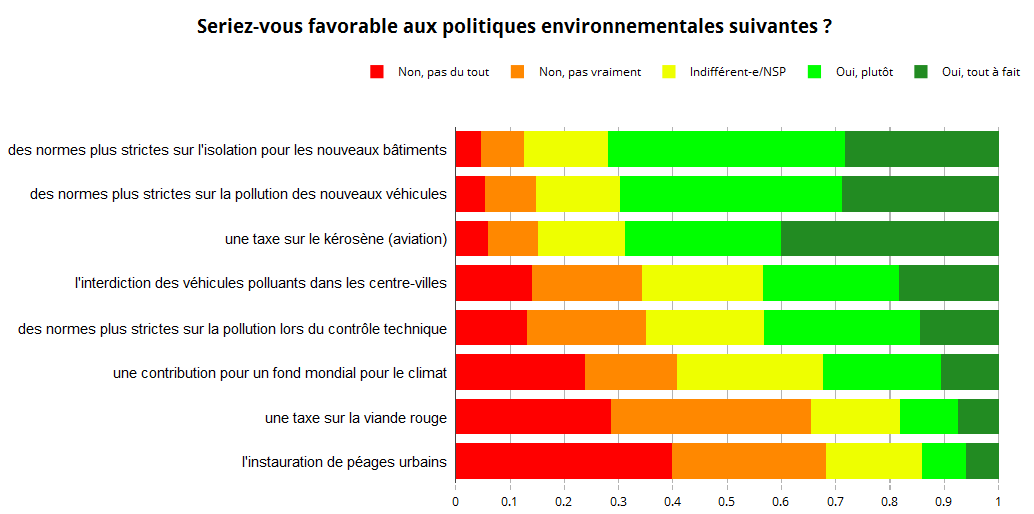
\includegraphics[width=0.95\columnwidth]{images/politiques_environnementales}
\end{figure}
\begin{figure}[H]
\centering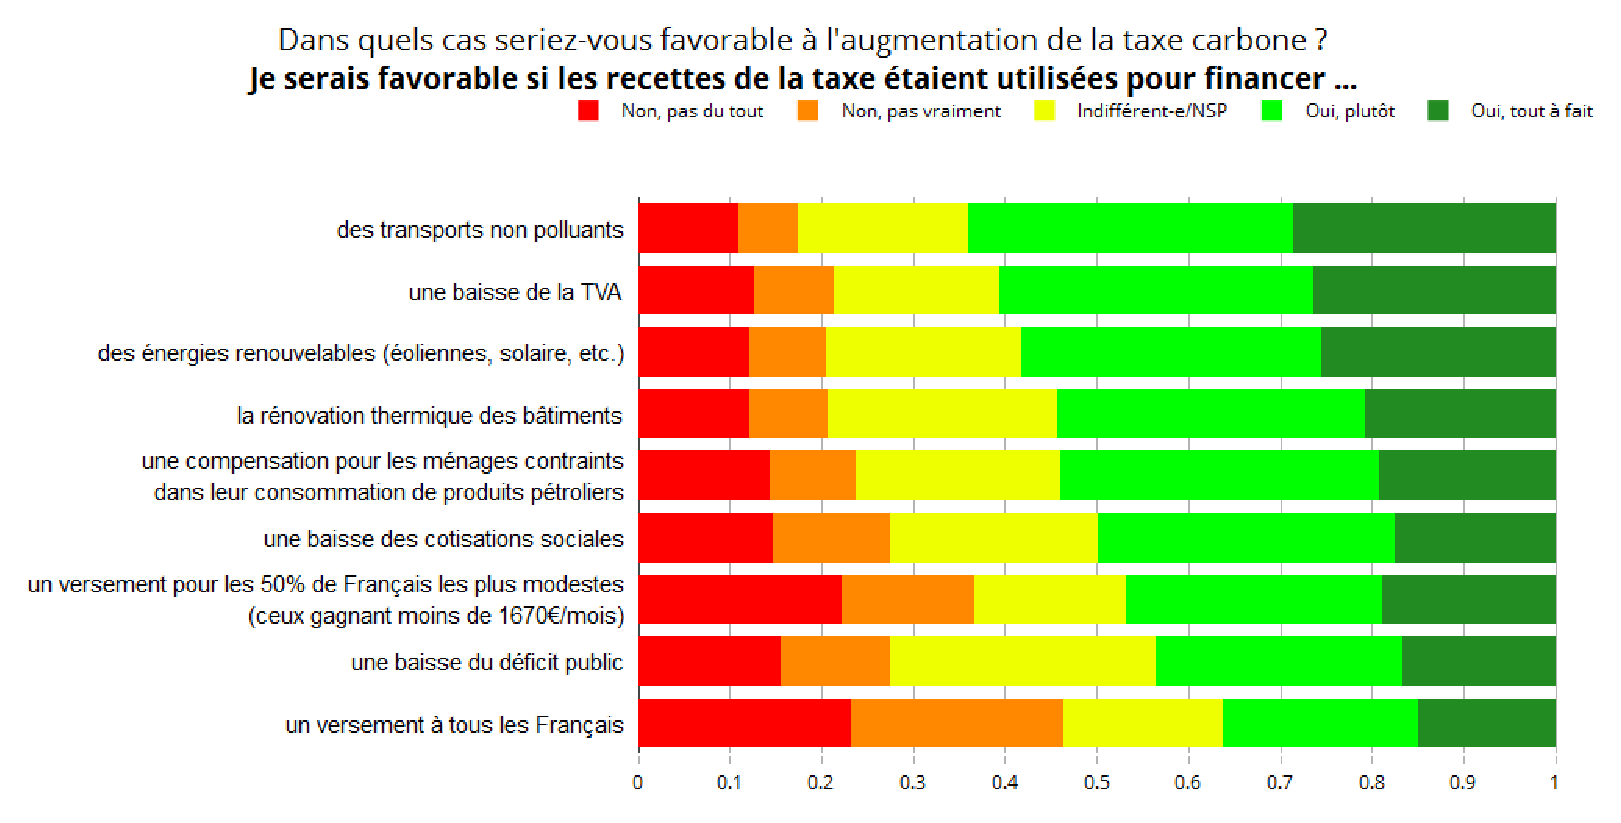
\includegraphics[width=1\columnwidth]{images/taxe_condition}
\end{figure}

\selectlanguage{english}%
\begin{figure}[h]
\selectlanguage{french}%
\makebox[\textwidth][c]{\foreignlanguage{english}{}\subfloat{\selectlanguage{english}%
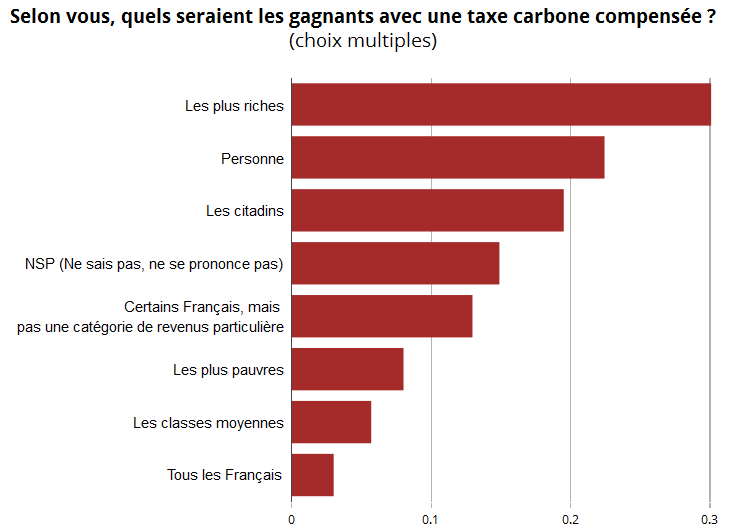
\includegraphics[width=0.55\columnwidth]{images/gagnants}\selectlanguage{french}%
}\foreignlanguage{english}{\qquad{}}\subfloat{\selectlanguage{english}%
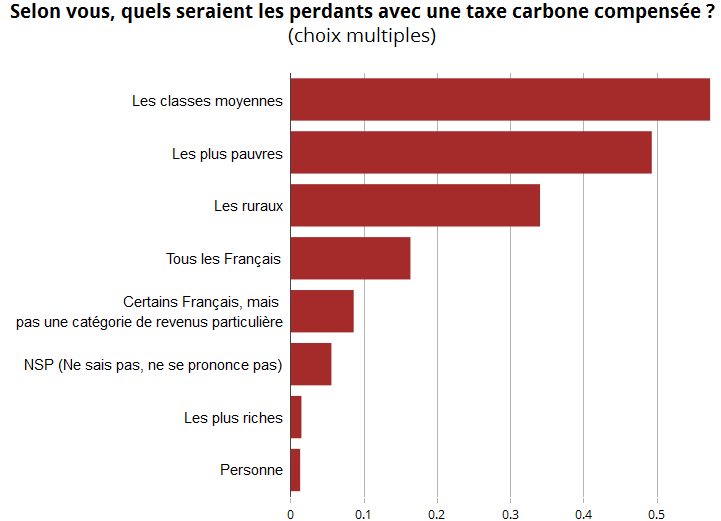
\includegraphics[width=0.55\columnwidth]{images/perdants}\selectlanguage{french}%
}\foreignlanguage{english}{}}\selectlanguage{english}%
\end{figure}
\begin{figure}
\centering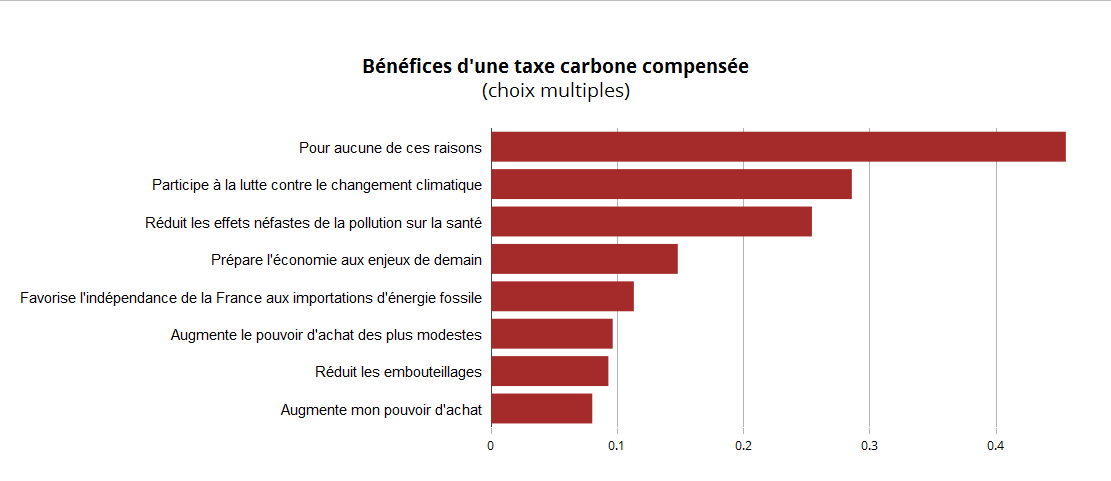
\includegraphics[width=1\columnwidth]{images/benefices}
\end{figure}
\begin{figure}
\centering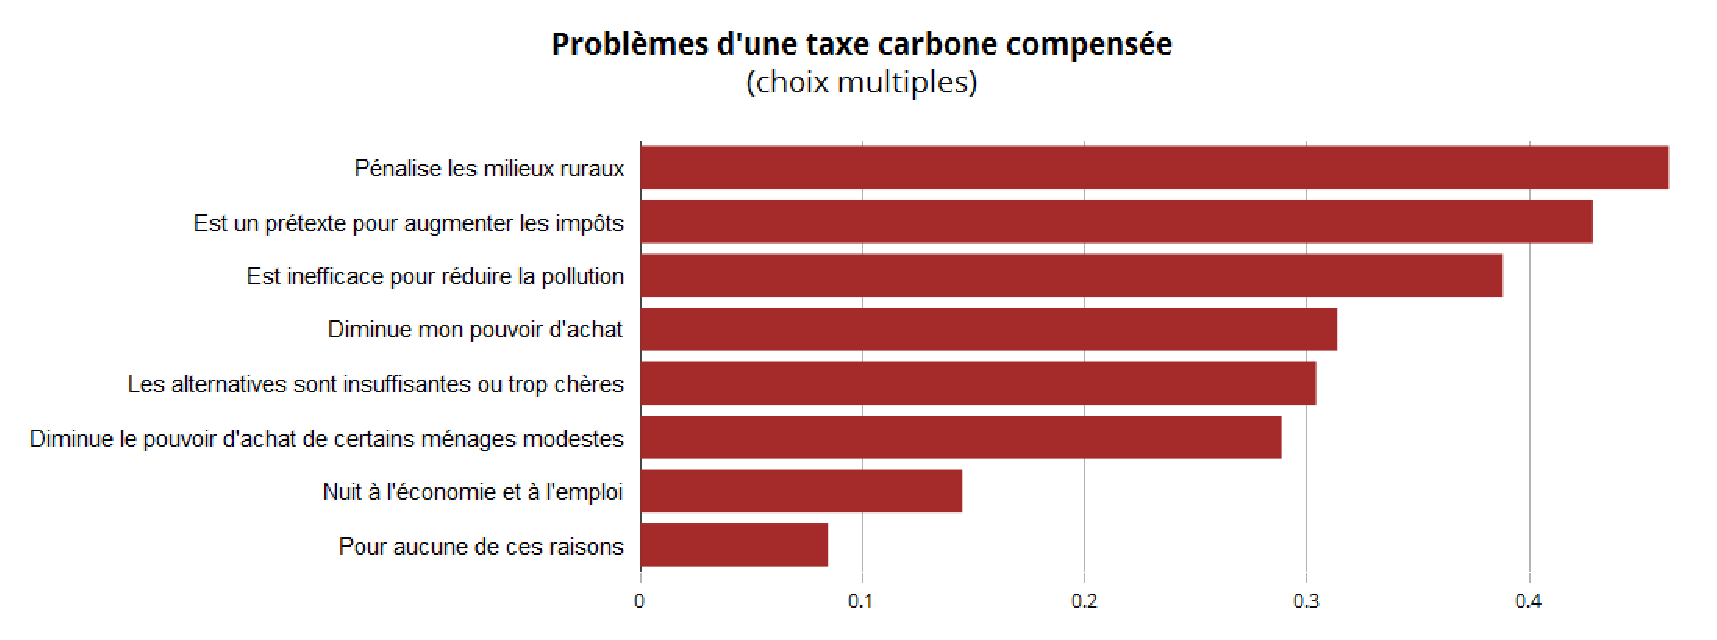
\includegraphics[width=1\columnwidth]{images/problemes}
\end{figure}

\selectlanguage{french}%
\begin{figure}
\centering\includegraphics[width=1\columnwidth]{\string"images/climat sondage automne 2016\string".eps}

\caption{R�sultats d'un sondage r�alis� � l'automne 2016 sur un �chantillon
repr�sentatif de 545 Fran�ais.}
\end{figure}

\end{document}
